\subsection{Rank lists fusion}
\label{sec:rank_lists_fusion}

The idea of rank list fusion is to combine multiple rank lists in such way that the resulting rank list is more accurate modelization of the real rank list.
The hypotetical best possible approximation of the real rank list in the case of authorship clustering is one such that  every true links (same authors document pairs) are at the top and every false links (different author document pairs) are at the bottom, therefore maximizing every metrics in Section~\ref{sec:rl_eval}.

\subsubsection{Z-Score fusion}

To merge scored rank list with differents order of magnitude, a simple and rather effective approach is to normalize every rank lists scores using the z-score (See Definition~\ref{def:z_score}) and then compute the merge rank list score for every link by taking the arithmetic mean of the same link score for every normalized rank lists.
This method can provide good results, but lack of theoretical foundations.
Example~\ref{ex:z_score_fusion} show an example for the z-score score fusion computation using two simple rank lists.

\begin{example}
  \caption{Z-Score fusion of two rank lists}
  \label{ex:z_score_fusion}

  \begin{subexample}{\linewidth}
    \centering
    \subcaption{Rank list A (Mean = 50, Std = 40.82)}
    \begin{tabular}{c l r r}
      \toprule
      Rank & Link name & Score & Z-Score \\
      \midrule
      1st & (0, 2) & $0$ & $-1.22$ \\
      2nd & (1, 2) & $50$ & $0$ \\
      3rd & (0, 1) & $100$ & $1.22$ \\
      \bottomrule
    \end{tabular}
  \end{subexample}

  \vspace{0.5cm}

  \textit{In this example, the scores does not satify the triangle inequality for the sake of simplicity.}

  \vspace{0.5cm}

  \begin{subexample}{\linewidth}
    \centering
    \subcaption{Rank list B (Mean = 0.33, Std = 0.17)}
    \begin{tabular}{c l r r}
      \toprule
      Rank & Link name & Score & Z-Score \\
      \midrule
      1st & (0, 2) & $0.1$ & $-1.37$ \\
      2nd & (0, 1) & $0.4$ & $0.39$ \\
      3rd & (1, 2) & $0.5$ & $0.98$ \\
      \bottomrule
    \end{tabular}
  \end{subexample}

  \vspace{0.5cm}

  \begin{subexample}{\linewidth}
    \centering
    \subcaption{Z-Score fusion}
    \begin{tabular}{c l r}
      \toprule
      Rank & Link name & Average Z-Score \\
      \midrule
      1st & (0, 2) & $(-1.22 + (-1.37)) / 2$ = $-1.30$ \\
      2nd & (1, 2) & $(0 + 0.98) / 2$ = $0.49$ \\
      3rd & (0, 1) & $(0.39 + 1.22) / 2$ = $0.81$ \\
      \bottomrule
    \end{tabular}
  \end{subexample}

\end{example}

\subsubsection{Regression fusion \label{sec:regression_fusion}}

Each rank list is ordered by a score, this score depends on distance measure used, thus the order of magnitude across rank list can different if they are generated with different distance measures.
To avoid this problem, the second solution is to translate the scores into a probability of being a true link.
To do so the logistic regression is used.
This method is similar to the one proposed in \textit{Le Calvé and Savoy (2000)}'s paper~\cite{le_calve_database_merging} and was used for merging rank list issued from information retrieval systems.

The main idea here is to learn a logistic regression model for each combination of text representation and distance metrics (here denoted \textit{type of rank list}).
From the rank list, a small feature vector for each link is created using : the log of the relative rank and the link score.
Since a probability of being a true link is desired, the target value for each link is either 1 for the true links or 0 when it's a false link.
One model per type of rank list is trained, this model can provide for any new same type rank list, probabilities for each link being of being a true link.

The probability framework can now be used on the rank list.
To obtain the most reliable probability given multiple observations (different rank lists), the regression fusion concists in computing the expected value for each link's probability using these observations.
In this case, the expected value is a simple average of the probabilities, since no weighting is used on the rank lists.

\subsubsection{Veto}

The idea here is to provide a veto power for the rank lists, to try to improve the results.
The following assumption is made: if a link have a low probability in a rank list before the fusion, this probably indicate a false link according to this rank list, thus having these links at the bottom of the rank list after the fusion can improve the results.

To fulfil the previously stated assumption, a possible way is to find every link in the ranks list before the fusion where the probability is under a certain threshold, and alter their probabilities (probability of being a true link) with $-\infty$.
Every links below the probability threshold will have its final score also equal to $-\infty$ since the average with any number and $-\infty$ is always $-\infty$.
When ordering the rank list, the links with a resulting $-\infty$ will subsequently be ranked at the bottom.

One problem arise with this solution, since multiple links can have a $-\infty$ probability, an order for these links is lost.
The proposed solution is to set the probability of the affected links to one of these values instead : $0$, $-1$ or $-n$, with $n = \#(ranks lists for the fusion)$.
The greater, the value, the stronger the penality of the veto.
The $-\infty$ method is the only real veto, in the first meaning of the veto definition, the other methods can be considered as a weighted veto.

Example~\ref{ex:veto} showcase an example where this method can provide better results.
As you can see with the rank lists in the example, rank list 1 give a 0.20 probability for link 4 of being a true link but rank list 3 give this link a 0.80 probability.
Without the veto the link is ranked 3rd but with the veto the link is ranked 5th tie with link 5.
The $-n$, method provide a why to avoid having tie and keep the strong impact of the $-\infty$ veto.
By setting to $0$, $-1$ or $-n$ can lightens the veto effect and conserve an order in the bottom rank links.

\begin{example}
  \centering
  \caption{Veto fusion}
  \label{ex:veto}

  \begin{subexample}{\linewidth}
    \centering
    \subcaption{Rank lists probabilites}
    \begin{tabular}{l l l}
      \toprule
      Rank list 1 & Rank list 2 & Rank list 3 \\
      \midrule
      0 : 0.95    & 0 : 0.90    & 5 : 0.90 \\
      1 : 0.75    & 3 : 0.70    & 4 : 0.80 \\
      2 : 0.60    & 4 : 0.65    & 0 : 0.70 \\
      3 : 0.50    & 1 : 0.50    & 1 : 0.60 \\
      4 : 0.20    & 2 : 0.30    & 2 : 0.50 \\
      5 : 0.10    & 5 : 0.10    & 3 : 0.40 \\
      \bottomrule
    \end{tabular}
  \end{subexample}

  \vspace{0.5cm}

  \begin{subexample}{\linewidth}
    \centering
    \subcaption{Rank list average link probability without veto}
    \begin{tabular}{l l l}
      \toprule
      Rank & Link: Average \\
      \midrule
      1st & 0 : $(0.95 + 0.90 + 0.70)/3 = 0.85$ \\
      2nd & 1 : $(0.75 + 0.50 + 0.60)/3 = 0.62$ \\
      3rd & 4 : $(0.20 + 0.65 + 0.80)/3 = 0.55$ \\
      4th & 3 : $(0.50 + 0.70 + 0.40)/3 = 0.53$ \\
      5th & 2 : $(0.60 + 0.30 + 0.50)/3 = 0.47$ \\
      6th & 5 : $(0.10 + 0.10 + 0.90)/3 = 0.37$ \\
      \bottomrule
    \end{tabular}
  \end{subexample}

  \vspace{0.5cm}

  \begin{subexample}{\linewidth}
    \centering
    \subcaption{$-\infty$ veto with threshold at 0.25}
    \begin{tabular}{l l l}
      \toprule
      Rank list 1 & Rank list 2 & Rank list 3 \\
      \midrule
      0 : 0.95    & 0 : 0.90    & 5 : 0.90 \\
      1 : 0.75    & 3 : 0.70    & 4 : 0.80 \\
      2 : 0.60    & 4 : 0.65    & 0 : 0.70 \\
      3 : 0.50    & 1 : 0.50    & 1 : 0.60 \\
      4 : -inf    & 2 : 0.30    & 2 : 0.50 \\
      5 : -inf    & 5 : -inf    & 3 : 0.40 \\
      \bottomrule
    \end{tabular}
  \end{subexample}

  \vspace{0.5cm}

  \begin{subexample}{\linewidth}
    \centering
    \subcaption{Rank list average link probability and $-1$ veto}
    \begin{tabular}{l l l}
      \toprule
      Rank & Link: Average \\
      \midrule
      1st & 0 : $(0.95 + 0.90 + 0.70)/3 = 0.85$ \\
      2nd & 1 : $(0.75 + 0.50 + 0.60)/3 = 0.62$ \\
      3rd & 3 : $(0.50 + 0.70 + 0.40)/3 = 0.53$ \\
      4th & 2 : $(0.60 + 0.30 + 0.50)/3 = 0.47$ \\
      5-6th & 4 : $(-inf + 0.65 + 0.80)/3 = -inf$ \\
      5-6th & 5 : $(-inf + -inf + 0.90)/3 = -inf$ \\
      \bottomrule
    \end{tabular}
  \end{subexample}
\end{example}

\subsubsection{Soft-veto using S-Curve}

As an extension to the veto method, an additional desired constraint is to favour top ranked link and as well as penalizing bottom ranked links like the veto method when fusing rank lists.
This constraint can be easily explained by observing the distance over the rank graph of the rank list.
Figure~\ref{fig:distance_over_rank} clearly show us the top ranked links and bottom ranked links have a sharper difference in distance than in than the middle section.

Top ranked links correspond to similar documents and bottom links correspond to negatively correlated documents.
Assuming that the top rank are true links after the rank list fusion these link should also be top rank.
The same reasoning can be applied for the bottom links by assuming them as false links.
A weighting curve, here called soft-veto, can be design accordingly such that the score of top links are boosted, and bottom links score hindered.

Using the reciprocal of the sigmoid function, such a curve can modelize.
Equation~\ref{eq:sigmoid} and~\ref{eq:sigmoid_r}.

\begin{equation}
  \label{eq:sigmoid}
  S(x) = \frac{1}{1+e^{-x}}
\end{equation}
\begin{equation}
  \label{eq:sigmoid_r}
  S^{-1}(x) = -\ln{\frac{x-1}{x}}
\end{equation}

The steepness of the curve can be adjusted by changing the start and the end of the interval and then normalizing the values between -1 and 1.
Figure~\ref{fig:s_curve_c} shows the $S^-1(x)$ function normalized between -1 and 1 for the intervals between $\lim\limits_{c \rightarrow 0} \left[S(c), S(c)\right]$ and $\left[S(-20), S(+20)\right]$.
A greater interval size increases the steepness which correspond to an increase of the rank conservation of the top and bottom ranked links and decreasing the rank conservation of the middle ranked links, this corresponds to geometrical zoom in and out of the curve.
To break the symmetry for the curve, to be able to increase the conservation of the top rank while decreasing the conservation of the bottom ranked.
The solution proposed is to add a new parameter $r$, then take $r \cdot N$ samples for $\left[S(-c), S(0)\right]$ and $(1-r) \cdot N$ samples for $\left[S(0), S(c)\right]$.
Breaking the symmetry with this technique creates a non-derivable point at $r$, but it's not a problem for the current use.
Figure~\ref{fig:s_curve_r} shows the r parameter influance of a sigmoid with $c = 4$ and $r \in \left[0.1, 0.9\right]$.
The $c$ parameter must be in the interval $\left]0, \infty\right[$.
With a value close to $0$, the soft-veto have a weak effect.
with a large value, for example 20, the soft veto has a strong effect on the top and bottom, see Figure~\ref{fig:s_curve_c}.
The $r$ parameter must be in the interval $\left]0, 1\right[$.
With a value close to $0$ the soft-veto have a strong effect on the top ranked links.
With a large value a strong effect on the bottom ranked links, see Figure~\ref{fig:s_curve_r}.

To apply the soft-veto, each score in the rank list is multiplied by the s-curve at the same rank.
This soft-veto methodology aimed to be used on rank list before fusing, to have a more cleaved decision on the links positions.
This stragegy can be use on any type of scoring method (z-score scores or probabilites).

\begin{figure}
  \centering
  \caption{Distance over rank in the rank list using the smoothed Manhattan distance, 500 MFW tokens on the Brunet dataset}
  \label{fig:distance_over_rank}
  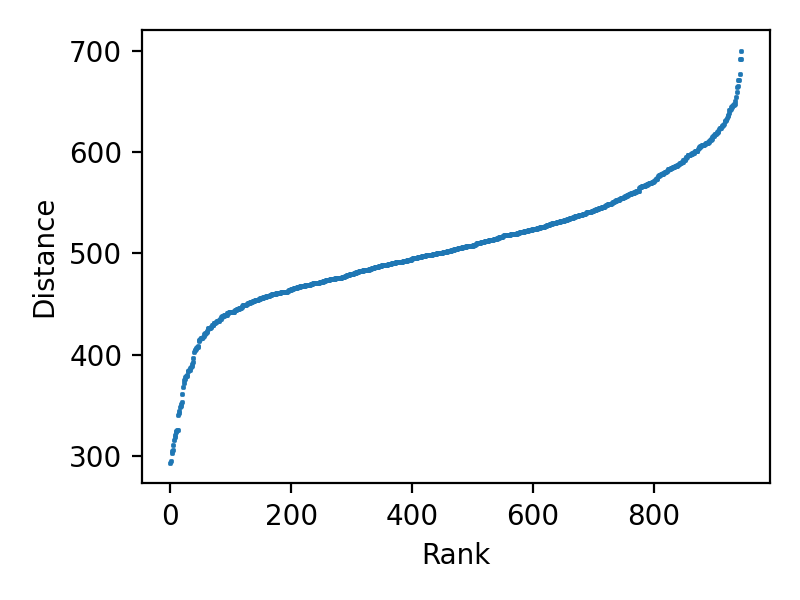
\includegraphics[width=\linewidth]{img/distance_over_rank.png}
\end{figure}

\begin{figure}
  \centering
  \caption{S-Curves parameters}
  \label{fig:s_curve_params}

  \subcaption{$S^-1(x)$, sampled in $\left[S(-c), S(+c)\right]$ and normalized between -1 and 1}
  \label{fig:s_curve_c}
  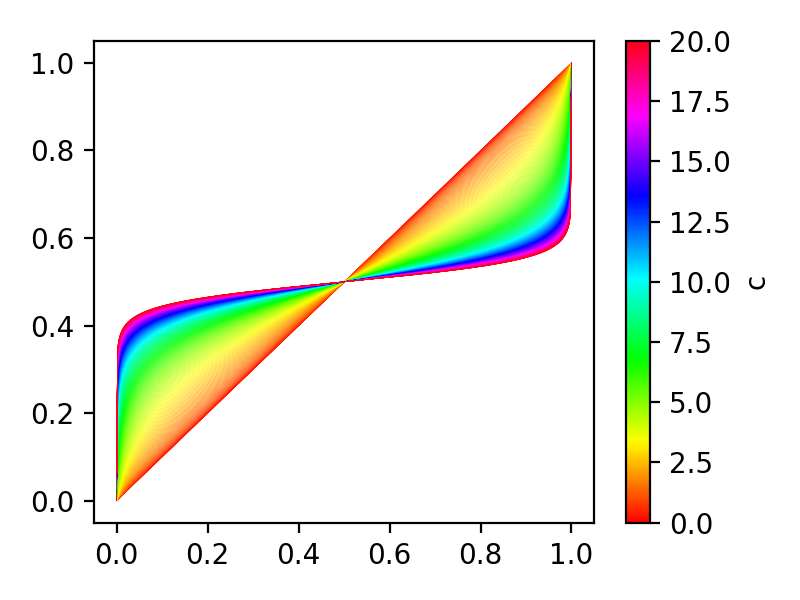
\includegraphics[width=\linewidth]{img/s_curve_c.png}

  \vspace{0.5cm}

  \subcaption{Sampling $S^-1(x)$ with $r \cdot N$ samples for $\left[S(-c), S(0)\right]$ and $(1-r) \cdot N$ samples for $\left[S(0), S(c)\right]$}
  \label{fig:s_curve_r}
  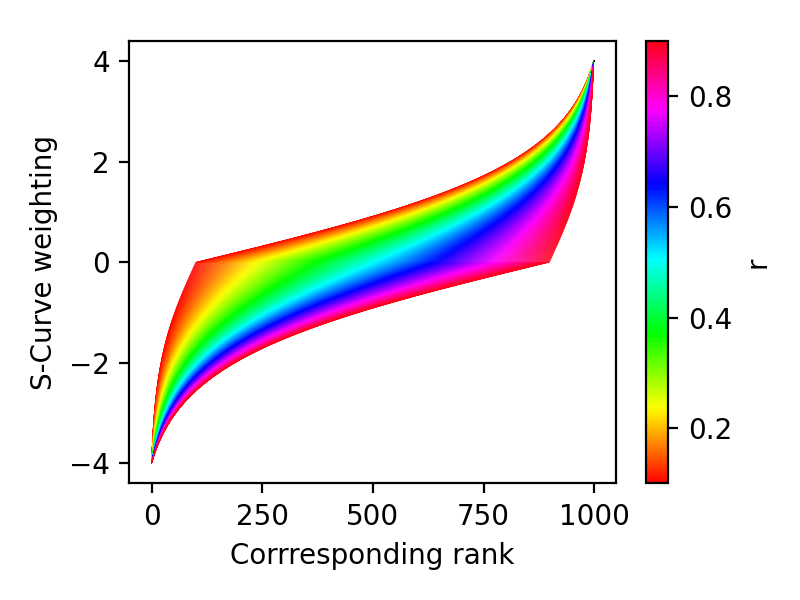
\includegraphics[width=\linewidth]{img/s_curve_r.png}

  \vspace{0.5cm}

  \subcaption{Example of S-curve with $c=4$ and $r=0.85$}
  \label{fig:s_curve_example}
  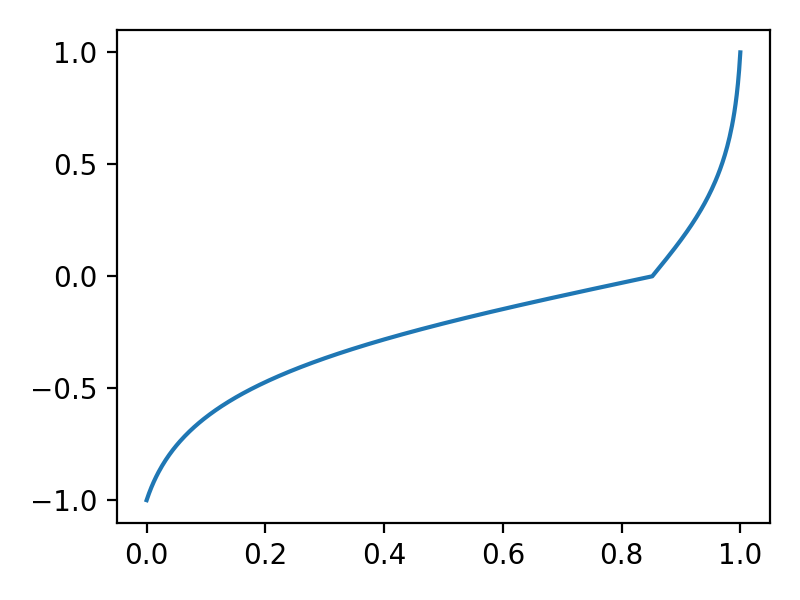
\includegraphics[width=0.9\linewidth]{img/s_curve_example.png}
\end{figure}
